\documentclass{sig-alternate-eEnergy_v2} 
%\documentclass{acm-alternate} 
%\documentclass{acm} 
%\documentclass[conference]{acm} 
%\documentclass[conference]{IEEEtran} 
%\documentclass[10pt,conference]{IEEEtran} 
\usepackage{graphicx}
\usepackage{subfigure}
\usepackage{epsfig}
\usepackage{amssymb,amsfonts,amsmath,amsthm}
\usepackage{verbatim}
\usepackage{moreverb}
\usepackage{rotating}
\usepackage{algorithmic}
\usepackage{epstopdf}
\usepackage{color}

%\usepackage{epstopdf}
%\usepackage{amsmath}
\DeclareGraphicsRule{.tic}{png}{.png}{`convert #1 `dirname #1`/`basename #1 .tif`.png}


\newtheorem{theorem}{Theorem}[section]
\setcounter{theorem}{0}
\newtheorem{algorithm}[theorem]{Algorithm}
\newtheorem{claim}[theorem]{Claim}
\newtheorem{conjecture}[theorem]{Conjecture}
\newtheorem{corollary}[theorem]{Corollary}
\newtheorem{fact}[theorem]{Fact}
\newtheorem{lemma}[theorem]{Lemma}
\newtheorem{meta-proposition}[theorem]{Meta-Proposition}
\newtheorem{note}[theorem]{Note}
\newtheorem{observation}[theorem]{Observation}
\newtheorem{proposition}[theorem]{Proposition}
\newtheorem{proviso}[theorem]{Proviso}         
\newtheorem{question}[theorem]{Question}         
\newtheorem{remark}[theorem]{Remark}         
\newtheorem{define}[theorem]{Definition}         

%\newcommand{\HRule}{\rule{\linewidth}{0.5mm}}
%\setlength\fboxsep{0pt}
%\setlength\fboxrule{0.5pt}


\newcommand{\sat}{{\textsc{P3SAT} }}
\newcommand{\sats}{{\textsc{P3SAT}}}
\newcommand{\full}{{\textsc{FullObserve} }}
\newcommand{\fulls}{{\textsc{FullObserve}}}
\newcommand{\maxinc}{{\textsc{MaxObserve} }}
\newcommand{\maxincs}{{\textsc{MaxObserve}}}
\newcommand{\xval}{{\textsc{FullObserve-XV} }}
\newcommand{\xvals}{{\textsc{FullObserve-XV}}}
\newcommand{\xvalpart}{{\textsc{MaxObserve-XV} }}
\newcommand{\xvalparts}{{\textsc{MaxObserve-XV}}}

\newcommand{\xxx}[1]{\textit{\textcolor{red}{[[#1]]}}} % this is an elisha comment
\newcommand{\yyy}[1]{\textcolor{blue}{#1}} % this is an elisha comment


\makeatletter
\newcommand{\un}[1]{%
    \ifmmode \@@underline{#1} \else %
             $\@@underline{\hbox{#1}}$\fi}
\makeatother
\raggedbottom

\newcommand{\doctitle}{On the Impact of PMU Placement on Observability and Cross-Validation} 



\begin{document}


\title{\doctitle}


\author{
\alignauthor Daniel Gyllstrom, Elisha Rosensweig, and Jim Kurose \\
\affaddr{Department of Computer Science. University of Massachusetts Amherst USA}  \\ 
\email{\{dpg, elisha, kurose\}@cs.umass.edu} 
}

\maketitle

%\section{Abstract}

\begin{abstract}

Malicious and misconfigured nodes can inject incorrect state into a distributed system, which can then be propagated system-wide as a result of normal network operation. 
Such false state can degrade the performance of a distributed system or render it unusable. For example, in the case of network routing algorithms, false state corresponding
to a node incorrectly declaring a cost of $0$ to all destinations (maliciously or due to misconfiguration) can quickly spread through the network. This causes other nodes to (incorrectly) 
route via the misconfigured node, resulting in suboptimal routing and network congestion. We propose three algorithms for efficient recovery in such scenarios, prove the correctness 
of each of these algorithms, and derive communication complexity bounds for each algorithm. Through simulation, we evaluate our algorithms -- in terms of message and time overhead -- when 
applied to removing false state in distance vector routing. Our analysis
shows that over topologies where link costs remain fixed and for the same topologies where link costs change, a recovery algorithm based on system-wide checkpoints and a rollback mechanism 
yields superior performance when using the poison reverse optimization.

\end{abstract}
%We propose algorithms that allow distributed routing algorithms to efficiently recover from false state injected into the network.
%We prove the correctness of each algorithm and evaluate them when applied to distance vector routing. In this context, we evaluate the message and time complexity of each algorithm through simulation.

%{\bf Keywords}: {\it distributed algorithms, fault tolerance, routing, security}


\category{C.2.0}{General}{Security and protection}
%\category{F.2.0}{General}{Redundant Design}{Security and protection}
%\category{B.4.5}{Reliability, Testing, and Fault-Tolerance}{Redundant Design}

\terms{Reliability}

\keywords{smart grid, energy, PMU, NP-Complete, cross-validation}


\section{Introduction}
\label{sec:intro-pmu}

\begin{framed}
\xxxxn{TODO Notes from Proposal Defense:}
\begin{itemize}
        \item \xxxxn{Lixin: Approximation bounds using modularity/sub-modular functions.  } 
	
	\item \xxxxn{Lixin: mention in future work (may already do this) that with special topologies you may be able to find more efficient algorithms for PMU placement.}

	\item \xxxxn{State Aazami et al show that the approximation for greedy algorithm is $\Theta(n)$, under the assumption that all nodes are zero-injection.  }
\end{itemize}
\end{framed}
               


This chapter considers placing electric power grid sensors, called phasor measurement units (PMUs), to enable measurement error detection.
%\xx{move paragraph to Smart Grid Overview Chapterr}
Significant investments have been made to deploy PMUs on electric power grids worldwide. PMUs provide \emph{synchronized} voltage and current measurements at a sampling rate orders 
of magnitude higher than the status quo: $10$ to $60$ samples per second rather than one sample every $1$ to $4$ seconds.  This allows system operators to directly measure the state of the electric power grid in real-time, rather than 
relying on imprecise state estimation. Consequently, PMUs have the potential to enable
an entirely new set of applications for the power grid:  protection and control during abnormal conditions, real-time distributed control, postmortem analysis of system faults,
advanced state estimators for system monitoring, and the reliable integration of renewable energy resources \cite{Naspi10}.

%\xx{move paragraph to Smart Grid Overview Chapter}
An electric power system consists of a set of buses  -- electric substations, power generation centers, or aggregation points of electrical loads -- and transmission lines connecting those buses.
The state of a power system is defined by the voltage phasor -- the magnitude and phase angle of electrical sine waves -- of all system buses and the current phasor of all transmission lines.
PMUs placed on buses provide real-time measurements of these system variables.
However, because PMUs are expensive, they cannot be deployed on all system buses \cite{Baldwin93}\cite{LaRee10}. Fortunately, the voltage phasor at a system bus can, at times, 
be determined (termed {\it observed} in this thesis) even when a PMU is not placed at that bus, by applying Ohm's and Kirchhoff's laws
on the measurements taken by a PMU placed at some nearby system bus \cite{Baldwin93}\cite{Brueni05}. Specifically, with correct placement of enough PMUs at a subset of system buses, the entire system state can be determined. 

In this chapter, we study two sets of PMU placement problems.  The first problem set consists of \full and \maxincs, and considers maximizing the observability of the network via PMU placement. \full considers the minimum number of PMUs needed 
to observe all system buses, while \maxinc considers the maximum number of buses that can be observed with a given number of PMUs. 
A bus is said to be {\em observed} if there is a PMU placed at it or if
its voltage phasor can be calculated using Ohm's or Kirchhoff's Law.  Although \full is well studied \cite{Baldwin93,Brueni05,Haynes02,Mili90,Xu04}, existing work considers only networks consisting solely of zero-injection buses, 
an unrealistic assumption in practice,
while we generalize the problem formulation to include mixtures of zero and  non-zero-injection buses. Additionally, our approach for analyzing \full provides the foundation with which to present the other three new (but related) PMU placement problems.

The second set of placement problems considers PMU placements that support PMU error detection. PMU measurement errors have been recorded in actual systems \cite{Vanfretti10}. 
One method of detecting these errors is to deploy PMUs ``near'' each other, thus enabling them to {\em cross-validate} each-other's measurements. 
{\xvals} aims to minimize the number of PMUs needed to observe all buses while insuring PMU cross-validation, and {\xvalparts} computes the maximum number of observed buses for a given number of PMUs, while insuring PMU cross-validation.


We make the following contributions in this chapter: 
\begin{itemize}
    
	\item We formulate two PMU placement problems, which (broadly) aim at maximizing observed buses while minimizing the number of PMUs used. Our formulation extends previously studied systems by 
	considering both zero and non-zero-injection buses.

    \item We formally define graph-theoretic rules for PMU cross-validation. Using these rules, we formulate two additional PMU placement problems that seek to maximize 
	the number of observed buses while minimizing the number of PMUs used under the condition that the PMUs are cross-validated. 

    \item We prove that all four PMU placement problems are NP-Complete. This represents our most important contribution.

	\item Given the proven complexity of these problems, we evaluate heuristic approaches for solving these problems. For each problem, we describe a greedy algorithm, and prove that each greedy
	algorithm has polynomial running time.

	\item Using simulations, we evaluate the performance of our greedy approximation algorithms over synthetic and actual
	IEEE bus systems. We find that the greedy algorithms yield a PMU placement that is, on average, within $97\%$ optimal. Additionally, we find that 
	the cross-validation constraints have limited effects on observability: on average our greedy algorithm that places PMUs according to the cross-validation rules observes 
	only $5.7\%$ fewer nodes than the same algorithm that does not consider cross-validation.

\end{itemize}

The rest of this chapter is organized as follows. In Section \ref{sec:prelim} we introduce our modeling assumptions, notation, and observability and cross-validation rules. In Section \ref{sec:problem-analysis} we formulate and prove the complexity of our four PMU placement problems. Section \ref{sec:approx} presents the approximation algorithms for each problem and Section \ref{sec:simulations} considers our simulation-based evaluation. We conclude with a review of related work (Section \ref{sec:related-pmu}) 
and concluding remarks (Section \ref{sec:pmu-conclude}).


%\input{intuition}

\section{Preliminaries}
\label{sec:prelim}

In this section we introduce notation and underlying assumptions (Section \ref{subsec:notation-assume}), 
and define our observability (Section \ref{subsec:observe}) and cross-validation (Section \ref{subsec:xval-rules}) rules.

%Before starting our analysis, we detail the notation used in this document.

\subsection{Assumptions, Notation, and Terminology}
\label{subsec:notation-assume}

%Consistent with the conventions in \cite{Baldwin93,Brueni05,Abur06,Mili90,Xu04,Xu05}, we make the following two assumptions about PMU placements and buses. First, a PMU can only be placed on a bus.
%Second, a PMU on a bus measures the voltage phasor at the bus and the current phasor of all transmission lines connected to it. 

Consistent with the conventions in \cite{Baldwin93,Brueni05,Abur06,Mili90,Xu04,Xu05}, we make the following assumptions about PMU placements and buses. 
First, a PMU can only be placed on a bus.  Second, a PMU on a bus measures the voltage phasor at the bus and the current phasor of all transmission lines connected to it.

%\begin{enumerate}
%	\item A PMU can only be placed on a bus.
%	\item A PMU on a bus measures the voltage phasor at the bus and the current phasor of all transmission lines connected to it. 
%\end{enumerate}

We model a power grid as an undirected graph $G=(V,E)$.  Each $v \in V$ represents a bus.  A bus is either an electrical substation, a power generation center, or an 
aggregation of loads. $V=V_Z \cup V_I$, where $V_Z$ is the set of all zero-injection buses and $V_I$ is the set of all non-zero-injection buses.  A bus is zero-injection if it has no load nor generator \cite{Zhang10}.
All other buses are non-zero-injection.  For simplicity, we refer to non-zero-injection buses as injection buses in the remainder of the paper. 
Each $(u,v) \in E$ is a transmission line connecting buses $u$ and $v$.  Figure \ref{fig:example} is an example of a power system modeled as such an undirected graph.

\begin{figure}[t]
\centering
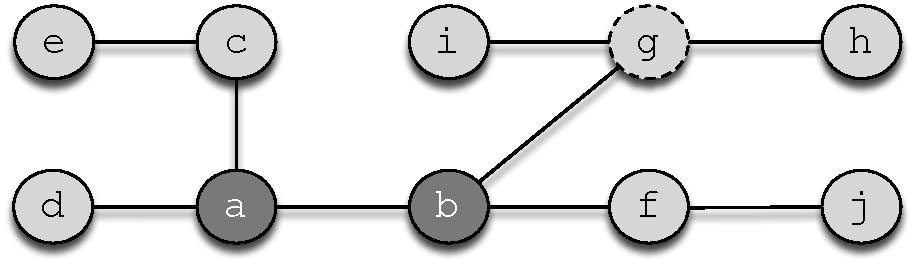
\includegraphics[scale=0.51]{figs/example4.pdf}
%\includegraphics[scale=0.51]{figs/example2.pdf}
\caption{Example power system graph. PMU nodes ($a,b$) are indicated with darker shading. Injection nodes have solid borders while zero-injection nodes  ($g$) have dashed borders.}
\label{fig:example}
\end{figure}

Using the same notation as Brueni and Heath \cite{Brueni05}, we define two $\Gamma$ functions. For $v\in V$ let $\Gamma(v)$ be the set of $v$'s neighbors in $G$, and $\Gamma[v] = \Gamma(v)\cup \{v\}$. 
% Since neighbor relationships are symmetric, $u\in\Gamma(v)\Rightleftarrow v\in\Gamma(u)$. 
A PMU placement $\Phi_G \subseteq V$ is a set of nodes at which PMUs are placed,
%We use the definition of a PMU placement from Brueni and Heath \cite{Brueni05}: a PMU cover, $\Phi$, is a subset of $V$ in which PMUs are placed such that all $v \in V$ and all $(u,v) \in E$ observed.
and $\Phi^R_G\subseteq V$ is the set of observed nodes for graph $G$ with placement $\Phi_G$ (see definition of observability below). %For convenience, we let $\Phi^R$ represent the observed nodes for graph $G$.
$k^* = \min \{|\Phi_G|:\Phi^R_G=V\}$ denotes the minimum number of PMUs needed to observe the entire network. Where the graph $G$ is clear from the context, we drop the $G$ subscript.
%Finally, $m$ is a constant corresponding to a graph $G=(V,E)$ such that $m < |V|$. 

%We let $\Phi^-$ represent the observed edges and $\Phi^R$ represent the observed nodes.
%All notation used in this document is shown in Table \ref{tab:notation}.

For convenience, we refer to any node with a PMU as a \emph{PMU node}. Additionally, for a given PMU placement we say that set $W\subseteq V$ is observed if all nodes in $W$ are observed, and if $W=V$ we refer to the graph as \emph{fully observed}. 


%%%%%%%%%%%%%%%%%%%%%%%%%%%%%%%%%%%%%%%%%%%%%%%%%%%%%%%%%%%%%%%%%%%% BEGIN COMMENT %%%%%%%%%%%%%%%%%%%%%%%%%%%%%%%%%%%%%%%%%%%%%%%%%%%%%%%%%%%%%%%%%%%%%%%%%%%%%%%%%%%%%%%%%%%%%%%%%%%%%%%%%%%%%%%%
\begin{comment}
\begin{table}[t]
\begin{center}
\begin{tabular}{l l} 
\hline \hline
   	{\bf Notation} & {\bf Meaning} \\
		  \hline 
		  	$G$ &  undirected graph $(V,E)$ where each $v \in V$ is a bus and each \\
				&  $(u,v) \in E$ is a transmission line connecting $u$ and $v$\\
			$\Gamma(v)$ & $\{u \in V$ $|$ $(u,v) \in E \}$ \\ 
			$\Gamma[v]$ & $\Gamma(v) \cup \{v\}$ \\
 		 	$n$ & $|V|$ \\
			$\Phi$ & a subset of $V$ in which PMUs are placed such that all \\ 
				   & $v \in V$ and all $(u,v) \in E$ observed  \\
			$\Phi^R$ & set of observed nodes \\
			$\Phi^-$ & set of observed edges \\
			\hline \hline
	\end{tabular}
	\end{center}
\caption{Notation Table}
\label{tab:notation}
\end{table}
\end{comment}
%%%%%%%%%%%%%%%%%%%%%%%%%%%%%%%%%%%%%%%%%%%%%%%%%%%%%%%%%%%%%%%%%%%% END COMMENT %%%%%%%%%%%%%%%%%%%%%%%%%%%%%%%%%%%%%%%%%%%%%%%%%%%%%%%%%%%%%%%%%%%%%%%%%%%%%%%%%%%%%%%%%%%%%%%%%%%%%%%%%%%%%%%%

\subsection{Observability Rules}
\label{subsec:observe}

We use the simplified observability rules elegantly formulated by Brueni and Heath \cite{Brueni05}.  We restate the rules here:  %which we restate here:  %For completeness, we restate the rules here:
%We use the simplified observability rules elegantly stated by Brueni and Heath \cite{Brueni05}, which we restate here:  %For completeness, we restate the rules here:
\begin{enumerate}
	
	\item {\bf Observability Rule 1 (O1)}.  {\it If node $v$ is a PMU node, then $\Gamma[v]$ is observed. Formally, if $v \in \Phi_G$, then $\Gamma[v] \subseteq \Phi^R_G$. }

	\item {\bf Observability Rule 2 (O2)}. {\it If a zero-injection node, $v$, is observed and  $\Gamma(v)\backslash\{u\}$ is observed for some $u\in\Gamma(v)$, then  $\Gamma[v]$ is observed.
	Formally, if $v \in \Phi^R_G \cap V_Z$ and $|\Gamma(v) \cap (V - \Phi^R_G)| \leq 1$, then $\Gamma[v] \subseteq \Phi^R_G$. }

\end{enumerate}

Consider the example in Figure \ref{fig:example}, where the shaded nodes are PMU nodes and $g$ is the only zero-injection node. 
%{\footnote {\small For all power system graphs shown in this document zero-injection nodes have a dashed border and injection nodes have a solid border.}}
Nodes $a-d$ are observed by applying O1 at the PMU at $a$, and nodes $a,b,f$ and $g$ are observed by applying O1 at $b$. 
$e$ cannot be observed via $c$ because $c$ does not have a PMU (O1 does not apply) and is an injection node (O2 does not apply). % so $e$ cannot be observed via $c$, which is its only neighbor. 
%$c$ does not have a PMU (O1 does not apply) and is an injection node (O2 does not apply), so $e$ cannot be observed via $c$, which is its only neighbor. 
Similarly, $j$ is not observed via $f$. Finally, although $g \in V_Z$, O2 cannot be applied at $g$ because $g$ has two unobserved neighbors $i,h$, so they remain unobserved.

Since O2 only applies with zero-injection nodes, more nodes are likely observed when nodes are zero-injection. For example, consider the case where $c$ and $f$ are {\em zero-injection} nodes. $a-d$, $g$ and $f$ are still observed as before, as O1 makes no 
conditions on the node type. Additionally, 
since $c,f \in V_Z$ and each has a single unobserved neighbor,  we can apply O2 at each of them to observe $e,j$, respectively. % making $e$ and $j$, respectively, observed.   
We evaluate the effect of increasing the number of zero-injection nodes on observability in our simulations (Section \ref{subsec:zero}).

%Finally, O2 can be applied at $e$ because $e \in V_Z$, $e$ is observed, and all of $e$'s neighbors except $i$ are observed. As a result, $i$ becomes observed. 
%Note that O2 cannot be applied at $f$ because $f$ has two unobserved neighbors. %This leaves $g$ and $h$ as the only two unobserved nodes in this example. 

%\begin{figure*}[t]
%  \begin{center}
%    \fbox{\subfigure[Case O1]{\label{fig:s1}\includegraphics[scale=0.28]{figs/s1.pdf}}}
%    \fbox{\subfigure[Case O2]{\label{fig:s2}\includegraphics[scale=0.28]{figs/s2.pdf}}} 
%  \end{center}
%	\caption{Rule Set 2} 
%  \label{fig:ruleset2}
%\end{figure*}




\subsection{Cross-Validation Rules}
\label{subsec:xval-rules}

% If phasor measured by 2 or more PMUs
From Vanfretti et al. \cite{Vanfretti10}, PMU measurements can be cross-validated when: (1) a 
voltage phasor of a non-PMU bus can be computed by PMU data from two different buses or (2) the current phasor of a transmission line can be computed from PMU data from two different buses. 
%Note that Vanfretti et al. \cite{Vanfretti10} use the term ``redundancy'' instead of cross-validation.  
{\footnote {\small  Vanfretti et al. \cite{Vanfretti10} use the term ``redundancy'' instead of cross-validation. }}  
Although it is the PMU data that is actually being cross-validated,
for convenience, we say a PMU is cross-validated. 
A PMU is \emph{cross-validated} if one of the rules below is satisfied \cite{Vanfretti10}: 
\begin{enumerate}
	
	\item {\bf Cross-Validation Rule 1 (XV1)}.  {\it If two PMU nodes are adjacent, then the PMUs cross-validate each other. % (Figure \ref{fig:validate}(a)). 
	Formally, if $u, v \in \Phi_G$, $u \in \Gamma(v)$, then the PMUs at $u$ and $v$ are cross-validated.}

	\item {\bf Cross-Validation Rule 2 (XV2)}. {\it If two PMU nodes have a common neighbor, then the PMUs cross-validate each other. % (Figure \ref{fig:validate}(b)). 
	Formally, if $u, v \in \Phi_G$, $u\neq v$ and $\Gamma(u)\cap\Gamma(v)\neq\emptyset$, then the PMUs at $u$ and $v$ are cross-validated.}
\end{enumerate}
In short, the cross-validation rules require that {\em the PMU is within two hops of another PMU}.
For example, in Figure \ref{fig:example}, the PMUs at $a$ and $b$ cross-validate each other by XV1. 

XV1 derives from the fact that both PMUs are measuring the current phasor of the transmission line connecting the two PMU nodes.  XV2 is more subtle.  
Using the notation specified in XV2, when computing the voltage phasor of an element in $\Gamma(u)\cap\Gamma(v)$ the voltage equations include variables to 
account for measurement error (e.g., angle bias) \cite{Vanfretti-thesis}. %\cite{Vanfretti10}.
When the PMUs are two hops from each other, there are more equations than unknowns, allowing for measurement error detection. 
Otherwise, the number of unknown variables exceeds the number of equations, which eliminates the possibility of detecting measurement errors \cite{Vanfretti-thesis}.
%Otherwise, the number of unknown variables grows faster than the number of equations, which eliminates the possibility of detecting measurement errors \cite{Vanfretti-thesis}.

%XV1 derives from the fact that both PMUs are measuring the current phasor of the transmission line connecting the two PMU nodes.  XV2 is more subtle.
%Using the notation specified in XV2, when computing the voltage phasor of an element in $\Gamma(u)\cap\Gamma(v)$ the equations include variables to account for measurement error (e.g., angle bias).
%%In order to account for measurement error, the equations used to compute the voltage phasor of the neighbor node shared by the PMU nodes include varialbes to account
%%for measurement error. Computing the voltage phasor of the neighbor node shared by the two PMU nodes
%%When computing the voltage phasor of the common neighbor node shared by the PMU nodes the equations include variables to account for measurement error (e.g., angle bias).
%When the PMUs are two hops from each other, there are more equations than unknowns, allowing for measurement error detection.
%Otherwise, the number of unknown variables exceeds the number of equations, which eliminates the possibility of detecting measurement errors \cite{Vanfretti-thesis}.
%Otherwise, the number of unknown variables grows faster than the number of equations, which eliminates the possibility of detecting measurement errors \cite{Vanfretti-thesis}.






%\input{problem-stmt-long}
\section{Four NP-Complete PMU Placement Problems}
\label{sec:problem-analysis}

In this section we first define four PMU placement problems and then provide a high-level description of the proof strategy we use to prove each problem is NP-Complete.
\yyn{In all four problems defined in this paper, we are only concerned with computing the voltage phasors of each bus (i.e., observing the buses). 
Using the values of the voltage phasors, Ohm's Law can be easily applied to compute the current phasors of each transmission line.}
Also, we consider networks with both injection and zero-injection buses.


\subsection{Problem Statements}

Here we briefly define each of our four PMU placement problems: \fulls, \maxinc, \xvalparts, and \xvals. \\ 
{\bf \full Decision Problem:} \\
\indent \underline{Instance}: Graph $G=(V,E)$ where $V=V_Z \cup V_I$, $V_Z \neq \emptyset$, $k$ PMUs such that $k \geq 1$. \\
\indent \underline{Question}: Is there a $\Phi_G$ such that $|\Phi_G| \leq k$ and $\Phi^R_G = V$?  \\
{\bf \maxinc Decision Problem:} \\
\indent \underline{Instance}: Graph $G=(V,E)$ where $V=V_Z \cup V_I$, $k$ PMUs such that $1 \leq k < k^*$. \\
\indent \underline{Question}: For a given $m< |V|$, is there a $\Phi_G$ such that $|\Phi_G| \leq k$ and $m \leq |\Phi^R_G| < |V|$? \\
{\bf \xval Decision Problem:} \\
\indent \underline{Instance}: Graph $G=(V,E)$ where $V=V_Z \cup V_I$, $k$ PMUs such that $k \geq 1$. \\
\indent \underline{Question}: Is there a $\Phi_G$ such that $|\Phi_G| \leq k$ and $\Phi^R_G = V$ under the condition that each $v \in \Phi_G$ is cross-validated? \\
{\bf \xvalpart Decision Problem:} \\
\indent \underline{Instance}: Graph $G=(V,E)$ where $V=V_Z \cup V_I$, $k$ PMUs such that $1 \leq k < k^*$, and some $m<|V|$. \\
\indent \underline{Question}: Is there a $\Phi_G$ such that $|\Phi_G| \leq k$ and $m \leq|\Phi^R_G| < |V|$ under the condition that each $v \in \Phi_G$ is cross-validated?


\begin{theorem}
\maxincs, \xvalparts, \full and \xval are all NP-Complete.
\label{thm:pmu-npc}
\end{theorem}



\subsection{Overview of NPC Proof Strategy}
\label{subsec:proofstrat}
In this section, we outline the proof strategy we used in each of NP-Completeness proofs.  Due to space constraints we omit the actual NPC proofs. 
Our proofs follow a similar structure proposed by Brueni and Heath \cite{Brueni05}. The authors prove NP-Completeness by reduction from planar 3-SAT (\sats).
A 3-SAT formula, $\phi$, is a boolean formula in conjunctive normal form (CNF) such 
that each clause contains at most $3$ literals. For any 3-SAT formula $\phi$ with the sets of variables $\{v_1,v_2, \dots , v_r\}$ and clauses $\{c_1,c_2, \dots , c_s \}$, $G(\phi)$ 
is the bipartite graph $G(\phi)=(V(\phi),E(\phi))$ defined as follows:
\begin{eqnarray*}
 V(\phi) &= &\{v_i\; \vert\; 1 \leq i \leq r \} \cup \{c_j \;\vert\; 1 \leq j \leq s \} \\
 E(\phi) &=& \{ (v_i,c_j)\;\vert\; v_i \in c_j\;\; or \;\; \overline{v_i} \in c_j\}.
\end{eqnarray*}
Note that edges pass only between $v_i$ and $c_j$ nodes, and so the graph is bipartite.  \sat is a 3-SAT formula such that $G(\phi)$ is planar \cite{Lich82}. 
For example, \sat formula
	 $\varphi = (\overline{v_1} \vee v_2 \vee v_3) \wedge (\overline{v_1} \vee \overline{v_4} \vee v_5) \wedge (\overline{v_2} \vee \overline{v_3} \vee \overline{v_5}) 
	 \wedge (v_3 \vee \overline{v_4}) \wedge  (\overline{v_3} \vee v_4 \vee \overline{v_5})$
has graph $G(\varphi)$ shown in Figure \ref{fig:gvarphi}. 
Discovering a satisfying assignment for  \sat is an NPC problem, and so it can be used in a reduction to prove the complexity of the problems we address here. 

Following the approach in \cite{Brueni05}, for \sat formula, $\phi$, we replace each variable node and each clause node in $G(\phi)$ with a specially constructed set of nodes,
termed a {\em gadget}. In this work, all variable gadgets will have the same structure, and all clause gadgets have the same structure (that is different from the variable gadget structure), 
and we denote the resulting graph as $H(\phi)$. In $H(\phi)$, each {\em variable} gadget has a subset of nodes that semantically represent assigning ``True" to that variable, and a subset of 
nodes that represent assigning it ``False". When a PMU is placed at one of these nodes, this is interpreted as assigning a truth value to the \sat variable corresponding with that gadget. 
Thus, we use the PMU placement to determine a consistent truth value for each \sat variable. Also, clause gadgets are connected to variable gadgets at either ``True" or ``False" (but never both) 
nodes, in such a way that the clause is satisfied if and only if {\em at least one} of those nodes has a PMU.

%While we assume $G(\phi)$ is planar, we make no such claim regarding $H(\phi)$, though in practice all graphs used in our proofs are indeed planar. The proof of NPC rests on the fact that 
%solving the underlying $\phi$ formula is NPC.

While the structure of our proofs is adapted from \cite{Brueni05}, the variable and clause gadgets we use to correspond to the \sat formula are novel, thus leading to a 
different set of proofs. Our work here demonstrates how the work in \cite{Brueni05} can be extended, using new variable and clause gadgets, to address a wide array of PMU placement problems.

\begin{figure}[t]

\subfigure[$G(\varphi)=(V(\varphi),E(\varphi))$ formed from $\varphi$ in Equation (\ref{eqn:varphi}).]{\label{fig:gvarphi}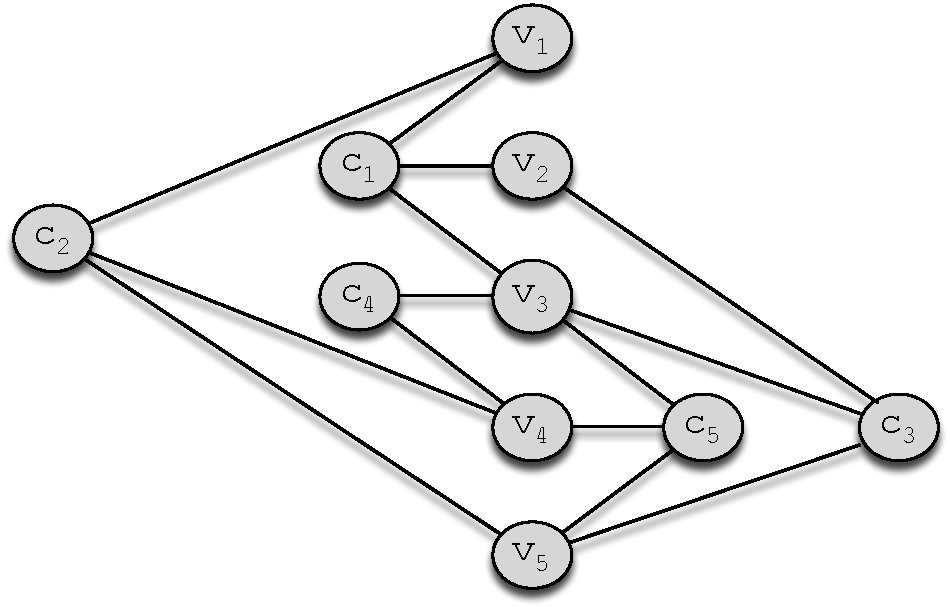
\includegraphics[scale=0.53]{figs/gvarphi.pdf}}
\subfigure[Graph formed using variable gadget from ...]{\label{fig:varphi2}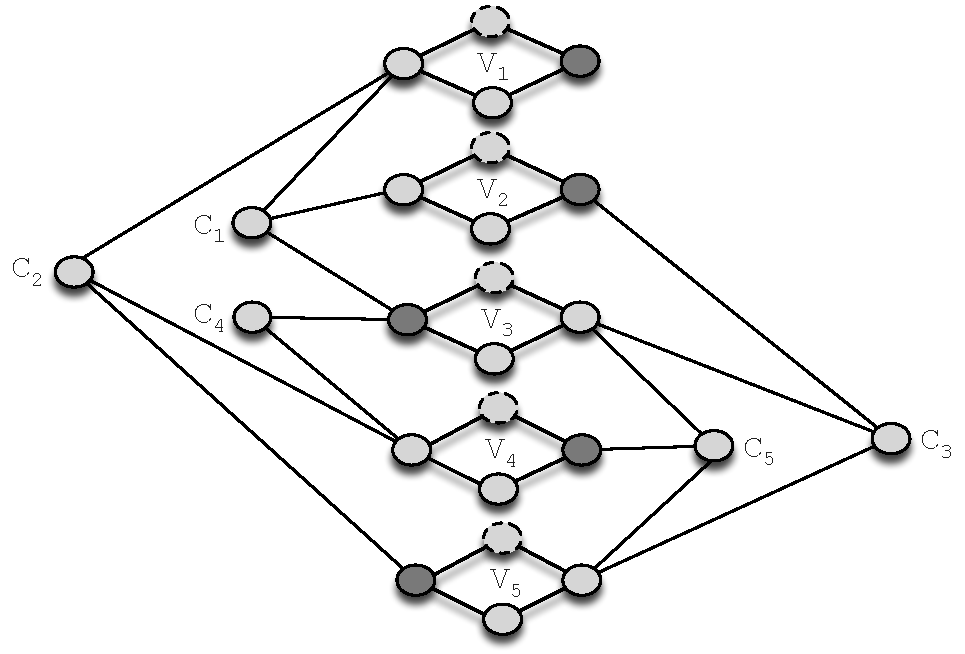
\includegraphics[scale=0.53]{figs/proof1-inject-example.pdf}}

\caption{Example } 
\end{figure}


\begin{figure}[t]
\centering
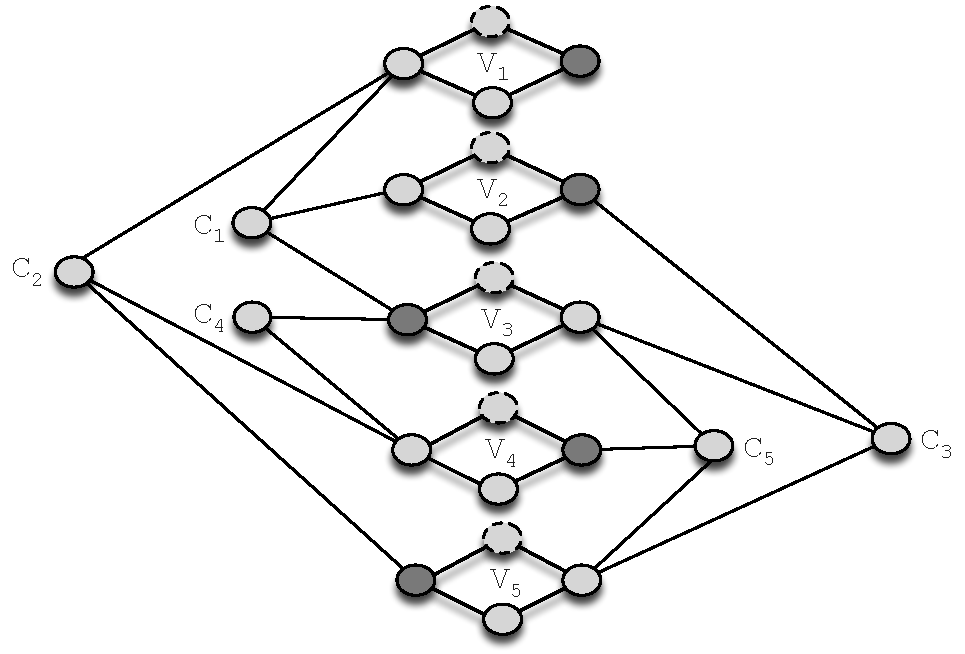
\includegraphics[scale=0.53]{figs/proof1-inject-example.pdf}
%\includegraphics[scale=0.51]{figs/example2.pdf}
\caption{Graph $G=(V,E)=H_1(\varphi)$ formed from $\varphi$ formula in Theorem \ref{thm:npc-full} proof. Nodes with a dashed border are zero-injection nodes.}
\label{fig:proof1-inject-example}
\end{figure}

\begin{figure}[t]
    \fbox{\subfigure[Variable gadget $V_i$ used in Theorem \ref{thm:npc-full} and Theorem \ref{thm:npc-maxinc}.]
	{\label{fig:diamond-gadget}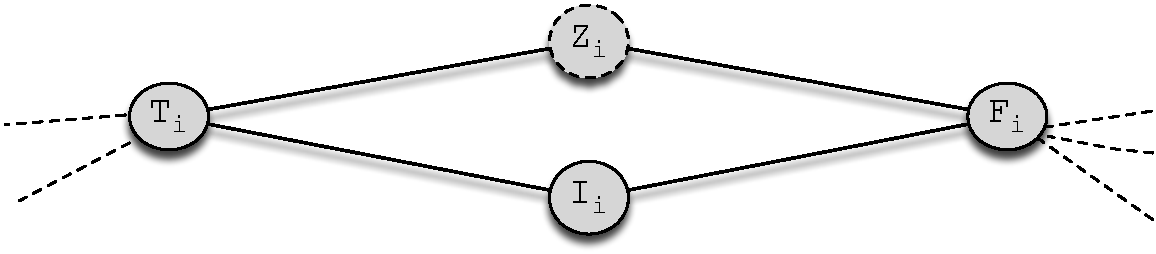
\includegraphics[scale=0.39]{figs/diamond-gadget.pdf}}}
    \fbox{\subfigure[Clause gadget $C_j$ used in Theorem \ref{thm:npc-maxinc}.]
	{\label{fig:line-gadget}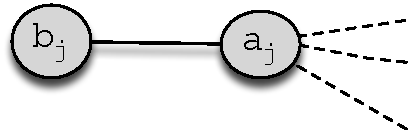
\includegraphics[scale=0.39]{figs/line-gadget.pdf}}}
	\caption{Gadgets used in Theorem \ref{thm:npc-full} and Theorem \ref{thm:npc-maxinc}. $Z_i$ in Figure (a) is the only zero-injection node. The dashed edges in Figure (a) are connections to clause gadgets.  Likewise, the dashed edges in Figure (b) are connections to variable gadgets. }
  \label{fig:pmu-gadgets}
\end{figure}


%\begin{figure}[t]
%\centering
%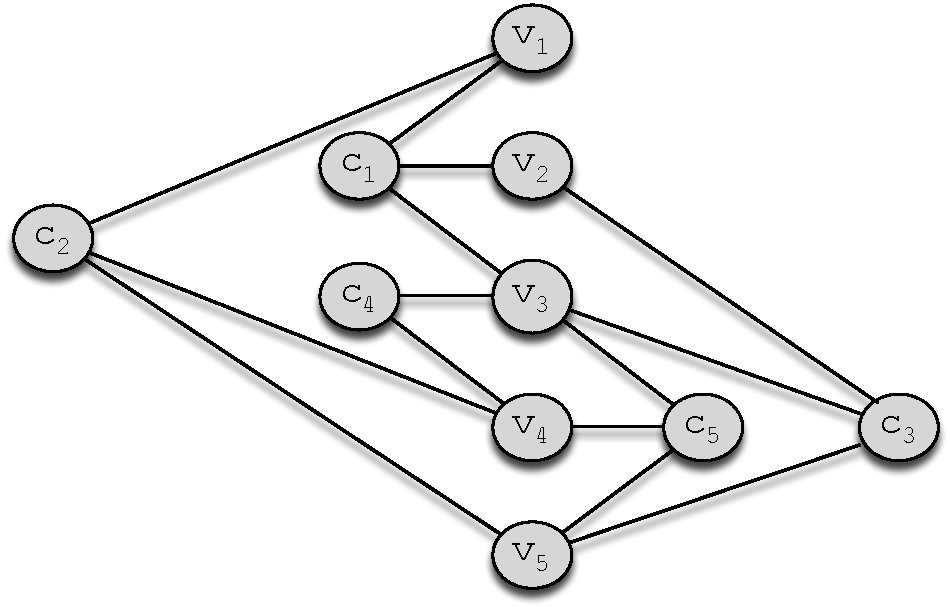
\includegraphics[scale=0.53]{figs/gvarphi.pdf}
%\caption{$G(\varphi)=(V(\varphi),E(\varphi))$ formed from $\varphi$ in Equation (\ref{eqn:varphi}). }
%\label{fig:gvarphi}
%\end{figure}





\section{Approximation Algorithms}
\label{sec:approx}

Because all four placement problems are NPC, we propose greedy approximation algorithms for each problem, which iteratively add 
a PMU in each step to the node that observes the maximum number of new nodes. We present two such algorithms, one that directly addresses \maxinc ({\tt greedy}) and the other 
\xvalpart ({\tt xvgreedy}). {\tt greedy} and {\tt xvgreedy} can easily be used to solve \full and \xvals, respectively, by selecting the appropriate $k$ value to ensure full observability.
We prove these algorithms have polynomial complexity (i.e., they are in $\mathcal{P}$), making them feasible tools for approximating optimal PMU placement.
Lastly, we explore the possibility that the PMU observability rules are submodular functions (Section \ref{subsec:submodular}).

\subsection{Greedy Approximations}
\label{sec:greedy-approx}

{\bf {\tt greedy} Algorithm}. We start with $\Phi = \emptyset$.  At each iteration, we add a PMU to the node that results in the observation of the maximum number of 
new nodes. The algorithm terminates when all PMUs are placed.  {\footnote {\small The same greedy algorithm is proposed by Aazami and Stilp \cite{Aazami07} and
is shown to  $\Theta(n)$ approximation ratio under the assumption that all nodes are zero-injection.}}
The pseudo-code for {\tt greedy} can be found in Appendix \ref{sec:appendix-approx} (Algorithm \ref{alg:greedy}).

\begin{theorem}
For input graph $G=(V,E)$ and $k$ PMUs {\tt greedy} has $O(dkn^3)$ complexity, where $n=|V|$ and $d$ is the maximum degree node in $V$.
\label{thm:greedy-complex}
\end{theorem}
\begin{proof}
The proof can be found in Appendix \ref{sec:appendix-approx} (Theorem \ref{thm:app-greedy-complex}).
\end{proof}

{\bf {\tt xvgreedy} Algorithm}. {\tt xvgreedy} is almost identical to {\tt greedy}, except that PMUs are added in pairs such that the selected pair observe
the maximum number of nodes under the condition that the PMU pair satisfy one of the cross-validation rules. 
We provide the pseudo code for {\tt xvgreedy} in Algorithm \ref{alg:xvgreedy}.
%We provide the pseudo code for {\tt xvgreedy} and prove that {\tt xvgreedy} has polynomial running time in our Technical Report \cite{Tech12}. 

%Our Technical Report \cite{Tech12} gives the pseudo code for {\tt greedy} and {\tt xvgreedy} and includes proofs
%that these algorithms have polynomial complexity, making them feasible tools for approximating optimal PMU placement. 

%\xxn{Aazami and Stilp prove {\tt greedy} has a $\Theta(n)$ approximation ratio under the assumption that all nodes are zero-injection.}
\begin{theorem}
For input graph $G=(V,E)$ and $k$ PMUs {\tt xvgreedy} has $O(kdn^3)$ complexity, where $n=|V|$ and $d$ is the maximum degree node in $V$.
\label{thm:xvgreedy-complex}
\end{theorem}
\begin{proof}
This theorem is proved in Appendix \ref{sec:appendix-approx} (Theorem \ref{thm:app-xvgreedy-complex}).
\end{proof}


\subsection{Observability Rules as Submodular Functions?}
\label{subsec:submodular}

Submodular functions are set functions with diminishing marginal returns: the value that each subsequent element adds decreases as the size of the input set increases. 
More formally, let $X$ be a ground set such that $|X|=n$. We define a set function on $X$ as $f: 2^X \rightarrow \mathbb{R}$.
Using the definition from Dughmi \cite{Dughmi09} %\footnote{\url{http://theory.stanford.edu/~shaddin/papers/submodular\_survey.pdf}}, %a set function $f: 2^X \rightarrow \mathbb{R}$ 
$f$ is \emph{submodular} if, for all $A,B \subseteq X$ with $A \subseteq B$, and for each $j \in X$,
\begin{eqnarray}
f(A \cup \{j\}) - f(A) &\geq& f(B \cup \{j\}) - f(B)
\end{eqnarray}
It has been shown that greedy algorithms admit a $1-1/e$ approximation of submodular functions \cite{Nem78}, where $e$ is the base of the natural logarithm. For this reason,
we aim to show that our observability rules are submodular.

%For the PMU placement problem, we define $f: 2^X \rightarrow \mathbb{R}$ on graph, $G=(V,E)$, as the number of observed nodes derived by placing a PMU at each $x \in X$.  
For the PMU placement problem, consider $G=(V,E)$.  For $S \subseteq V$ we define $f(S)$ as the number of observed nodes derived by placing a PMU at each $s \in S$.  
We prove that $f$ is not submodular for graphs containing zero-injection nodes (Theorem \ref{thm:submodular1}) but is submodular when restricted
to graphs with only injection nodes (Theorem \ref{thm:submodular2}).  


\begin{theorem}
\label{thm:submodular1}
$f$ is not submodular for graphs, $G_z$, with zero-injection nodes.
\end{theorem}

\begin{proof}
Let $G_z$ be the graph from Figure \ref{fig:submodular-counter}, $A=\{a\}$, and $B=\{a,b\}$. Then, %when evaluate the observed nodes we find:
%In this example we let $A=\{a\}$ and $B=\{a,b\}$. Then, %We show $f$ is not a submodular function
\begin{eqnarray*}
f(A \cup \{c\}) - f(A) &\stackrel{?}{\geq}& f(B \cup \{c\}) - f(B) \\
f(A \cup \{c\}) - 2 &\stackrel{?}{\geq}& f(B \cup \{c\}) - 3 \\
3-2 &\stackrel{?}{\geq}& 8 - 3 \\
1 &\stackrel{?}{\geq}& 5
\end{eqnarray*}
We conclude that $f$ is not submodular for $G_z$. % and therefore that our observability rules are not submodular functions.
\end{proof}

Note that in this example, O2 prevented us from meeting the criteria for submodular functions.  For PMU placement $B \cup \{c\}$, we were able to apply O2 at $e$, resulting in the observation of the
chain of nodes at the top of the graph.  However, we were unable to apply O2 for the PMU placement $A \cup \{c\}$.  This observation provides the motivation for our next Theorem (\ref{thm:submodular2}).
  
%It follows that $f(A)=2$ and $f(B)=3$. 

\begin{figure}[t]
\centering
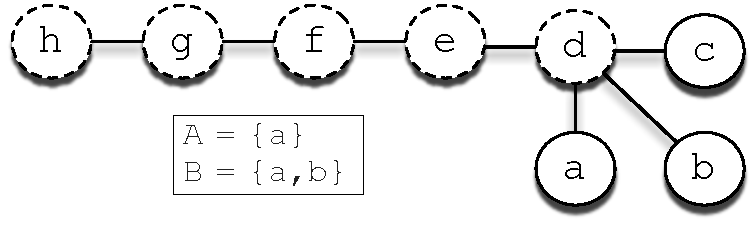
\includegraphics[scale=.75]{figs/submodular-counterexample.pdf}
\caption{Example used in Theorem \ref{thm:submodular1} showing a function defined using our observability rules is not submodular for graphs with zero-injection nodes.  
Nodes with a dashed border are zero-injection nodes and injection nodes have a solid border. For set function $f: 2^X \rightarrow \mathbb{R}$, defined as the number of observed nodes 
resulting from placing a PMU at each $x \in X$, we have $f(A) = f(\{a\}) = 2$ where $\{a,d\}$ are observed, while $f(B) = f(\{a,b\}) = 3$ where $\{a,b,d\}$ are observed.  }
\label{fig:submodular-counter}
\end{figure}


\begin{theorem}
\label{thm:submodular2}
$f$ is a submodular function for graphs, $G_I$, containing only injection nodes.
\end{theorem}

\begin{proof}
Consider a graph $G_I=(V_I,E_I)$ where each $v \in V_I$ is an injection node. Let $A \subseteq B \subseteq V_I$ and $j \in V_I$.  Placing a PMU at $j$ can at most result in the observation of
$j \cup \Gamma(j)$ because we cannot apply O2 in $G_I$ since we have assumed all nodes are injection nodes.
%Since all nodes are injection nodes we cannot use O2 to observe any nodes. and thus nodes can only be observed using O1.  By O1, $j$ and $\Gamma(j)$ are observed.  
We claim that any $x \in j \cup \Gamma(j)$ that is unobserved after placing a PMU at nodes in $B$ is not observed with the PMU placement derived from $A$.  $x$ is unobserved only if 
$x$ has no PMU nor if any $\Gamma(x)$ has a PMU.  Since $A \subseteq B$ and we have assumed $x$ is not observed using $B$, it must be the case that $x$ is not observed under $A$.
%Since $A \subseteq B$, we know that if any $x \in \Gamma(j)$ is unobserved after placing a PMU at nodes in $B$ that $x$ is not observed with the PMU placement derived from $A$. 
Since we have show that all unobserved nodes resulting from PMU placement $B$ must be unobserved under $A$, we conclude that $f(A \cup \{j\}) - f(A) \geq f(B \cup \{j\}) - f(B)$ 
and, therefore, $f$ is submodular for $G_I$.
\end{proof}

%\xxn{Maybe we can show it is a submodular function for certain distributions of zero-injection nodes.}


%\subsection{Example Showing Greedy is not a Submodular Function}
%
%Submodular definition from \footnote{\url{http://theory.stanford.edu/~jvondrak/CS369P-files/lec16.pdf}}.  Denote $f_A(i) = f(A+i) - f(A)$ the marginal value of $i$ with respect
%to $A$.  $f$ is submodular if for all $A \subseteq B \subseteq N$ and $i \in N \setminus B$, 
%$$ f_A(i) \geq f_B(i) $$
%
%
%Execution of {\tt greedy} using Figure \ref{fig:submodular-counter}:
%\begin{enumerate}
%	\item Add PMU to $d$.  As a result, $5$ nodes, $\{a,b,c,d,h\}$, are observed by applying O1 at $d$,  O2 cannot be applied.
%	
%	\item Add PMU to $f$.  As a result, $6$ nodes become observed $\{e,f,g,i,j,k\}$ by applying O1 at $f$ and then repeatedly applying O2 (first at $h$, then at $j$, and finally at $k$)
%
%\end{enumerate}
%
%
%\begin{figure*}[t]
%  \begin{center}
%    \subfigure[The original graph (without any PMUs).]{\label{fig:submodular-counter-step0}
%		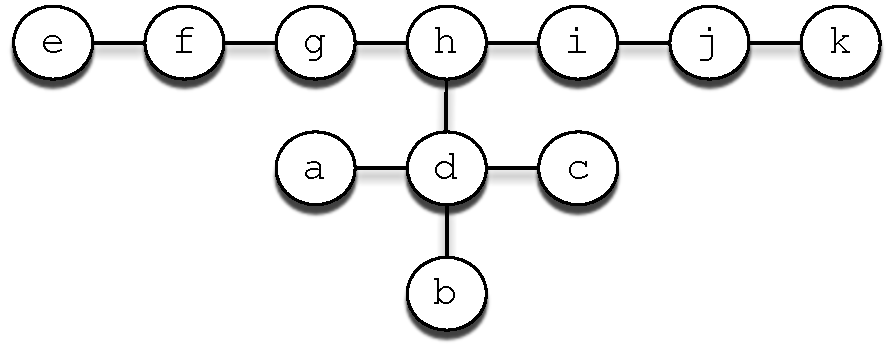
\includegraphics[scale=0.59]{figs/submodular-counterexample-step0.pdf}}
%    \subfigure[Step 1: Placing a PMU at $d$ results in the observation of $5$ nodes, $\{a,b,c,d,h\}$.]{\label{fig:submodular-counter-step1}
%		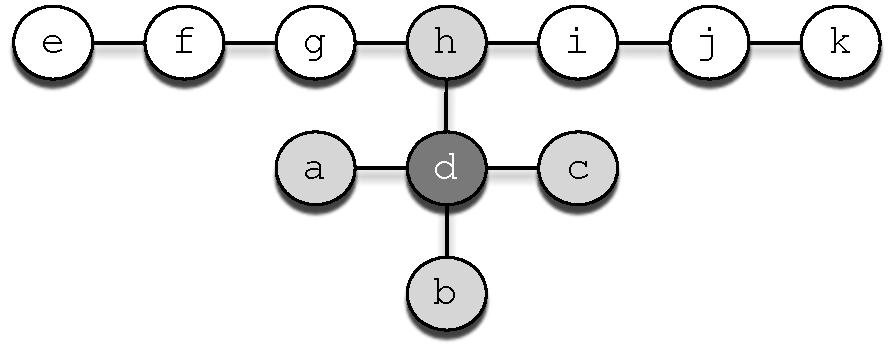
\includegraphics[scale=0.59]{figs/submodular-counterexample-step1.pdf}}
%    \subfigure[Step 2: Placing a PMU at $f$ results in the observation of $6$ nodes, $\{e,f,g,i,j,k\}$.]{\label{fig:submodular-counter-step2}
%		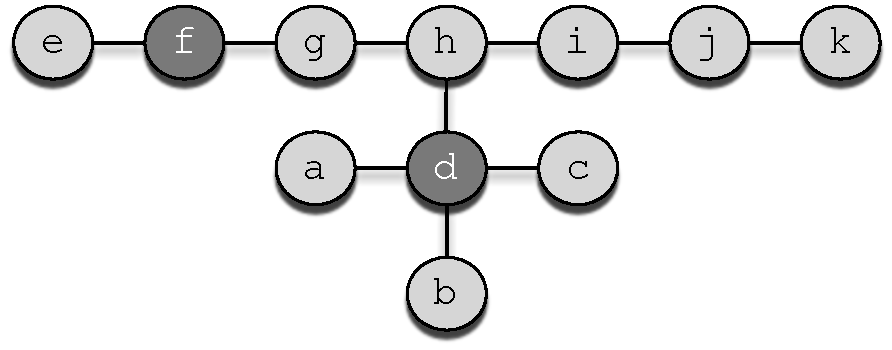
\includegraphics[scale=0.59]{figs/submodular-counterexample-step2.pdf}}
%  \end{center}
%	\caption{Example showing that {\tt greedy} is not a submodular function.} 
%	\label{fig:submodular-counter-old}
%\end{figure*}
%
%\end{comment}


%List of references explaining submodular functions.
%\footnote{Nice definition and examples. \url{http://theory.stanford.edu/~jvondrak/CS369P-files/lec16.pdf}}
%\footnote{Survey paper. \url{http://theory.stanford.edu/~shaddin/papers/submodular_survey.pdf}}
%\footnote{\url{http://en.wikipedia.org/wiki/Submodular_set_function}}
%\footnote{One of the earlier papers on submodular functions. \url{http://www.cs.toronto.edu/~eidan/papers/submod-max.pdf}}


 


\section{Simulation Study}
\label{sec:simulations}

\textbf{Topologies.} 
We evaluate our approximation algorithms with simulations over synthetic topologies generated using real portions of the North American electric power grid 
(i.e., IEEE bus systems $14$, $30$, $57$, and $118$) as templates \footnote{\url{http://www.ee.washington.edu/research/pstca/}}. 
The bus system number indicates the number of nodes in the graph (e.g., bus system $57$ has $57$ nodes).
It is standard practice in the literature to only use single IEEE bus systems \cite{Baldwin93,Abur06,Mili90,Xu04}.  
We follow this precedent but do not present these results because they are consistent with the trends found using synthetic topologies.
Instead, we focus on synthetic topologies because, unlike simulations using single IEEE bus systems, we can establish the statistical significance of the performance of our greedy approximations.

Since observability is determined by the connectivity of the graph, we use the {\em degree distribution} of IEEE topologies as the template for generating our synthetic graphs.
A synthetic topology is generated from a given IEEE graph by randomly ``swapping'' edges in the IEEE graph. Specifically, we select a random $v \in V$ and then pick a random $u \in \Gamma(v)$. 
Let $u$ have degree $d_u$.  Next, we select a random $w \notin \Gamma(v)$ with degree $d_w = d_u -1$. % {\footnote {\small Here ``random'' means uniformly at random.}
Finally, we remove edge $(v,u)$ and add $(v,w)$, thereby preserving the node degree distribution.
We continue this swapping procedure until the original graph and generated graph share {\em no edges}, and then return the resulting graph.

\textbf{Evaluation Methods.}
We are interested in evaluating how close our algorithms are to the optimal PMU placement. 
Thus, when computationally possible (for a given $k$) we use brute-force algorithms to iterate over all possible placements of $k$ PMUs in a given graph and select the best PMU placement. 
When the brute-force algorithm is computationally infeasible, we present only the performance of the greedy algorithm.
In what follows, the output of the brute-force algorithm is denoted {\tt optimal}, and when we require cross-validation it is denoted {\tt xvoptimal}.

%We consider performance as a function of the number of PMUs,
%We present three different simulations in Section \ref{subsec:synth}-\ref{subsec:ieee}. 
%In Section \ref{subsec:synth} we consider performance as a function of the number of PMUs, and
%in Section \ref{subsec:zero} we investigate the performance impact of the number of zero-injection nodes in the network.
%These two sections use synthetic graphs. We conclude in Section \ref{subsec:ieee}, where we compare these results to the performance over the actual IEEE graphs.

%\subsection{Simulation 1: Impact of Number of PMUs}
%\label{subsec:synth}

\textbf{Simulation Results.}
We vary the number of PMUs and determine the number of observed nodes in the synthetic graph. 
Each data point is generated as follows. For a given number of PMUs, $k$, we generate a graph, place $k$ PMUs on the graph, and then determine the number of observed nodes. 
We continue this procedure until $[0.9(\overline{x}),1.1(\overline{x})]$ -- where $\overline{x}$ is the mean number of observed nodes using $k$ PMUs -- falls within the $90\%$ confidence interval.

In addition to generating a topology, for each synthetic graph we determined the members of $V_I, V_Z$. These nodes are specified for the original graphs in the IEEE bus system database. Thus, 
we randomly map each node in the IEEE graph to a node in the synthetic graph with the same degree, and then match their membership to either $V_I$ or $V_Z$.

%We present here results for solving \maxinc and \xvalpart using synthetic graphs based on IEEE bus $57$.  
Due to space constraints, we only show plots for solving \maxinc and \xvalpart using synthetic graphs based on IEEE bus $57$.  
The number of nodes observed given $k$, using {\tt greedy} and {\tt optimal}, are shown in Figure \ref{fig:bus57}, and Figure \ref{fig:xvbus57} shows this number 
for {\tt xvgreedy} and {\tt xvoptimal}.  Both plots include the $90\%$ confidence intervals. 
Results for synthetic graphs generated using IEEE bus $14$, $30$, and $118$ yield the same trends.

Our greedy algorithms perform well. On average, {\tt greedy} is within $98.6\%$ of {\tt optimal},
is never below $94\%$ of {\tt optimal}, and in most cases gives the optimal result.
Likewise, {\tt xvgreedy} is never less than $94 \%$ of {\tt xvoptimal} and on average is within $97\%$ of {\tt xvoptimal}. In about about half the cases {\tt xvgreedy} gives the optimal result.
These results suggest that despite the complexity of the problems, a greedy approach can return high-quality results. Note, however, that these statistics do not include performance when
$k$ is large.  It is an open question whether {\tt greedy} and {\tt xvgreedy} would do well for large $k$. 

Surprisingly, when comparing our results with and without the cross-validation requirement, we find that the cross-validation constraints have little effect on the number of observed nodes 
for the same $k$. Our experiments show that on average {\tt xvoptimal} observed only $5\%$ fewer nodes than {\tt optimal}.  Similarly, on average {\tt xvgreedy} observes
 $5.7\%$ fewer nodes than {\tt greedy}. This suggests that the cost of imposing the cross-validation requirement is low, with the clear gain of ensuring PMU correctness across the network.


\begin{figure*}[t]
  \begin{center}
    \subfigure[{\tt greedy} vs {\tt optimal}]{\label{fig:bus57}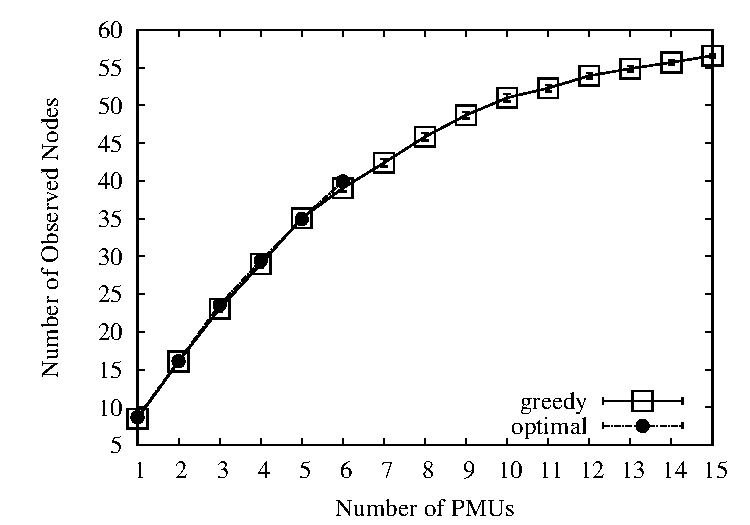
\includegraphics[scale=0.59]{figs/bus57.pdf}}
    \subfigure[{\tt xvgreedy} vs {\tt xvoptimal}]{\label{fig:xvbus57}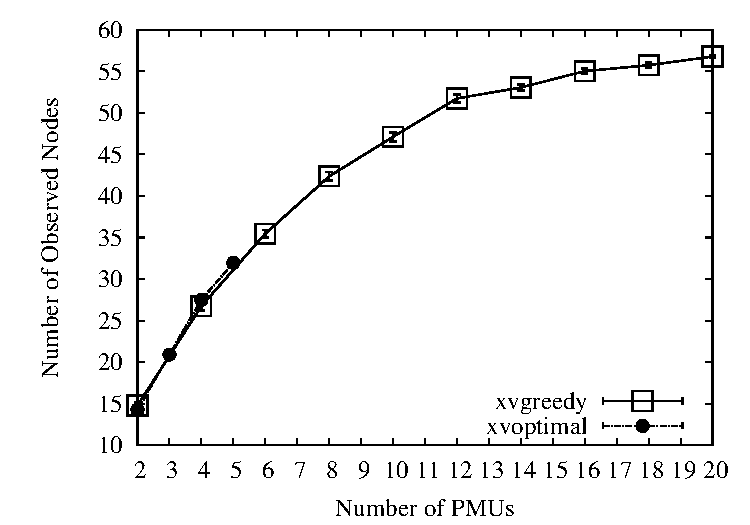
\includegraphics[scale=0.59]{figs/xvbus57.pdf}}
  \end{center}
	\caption{Mean number of observed nodes over synthetic graphs based on IEEE bus $57$ when varying number of PMUs. The $90\%$ confidence interval is shown.}
\end{figure*}








\section{Related Work}
\label{sec:related-pmu}

\full is well-studied \cite{Baldwin93,Brueni05,Haynes02, Mili90, Xu04}.  
Haynes et al. \cite{Haynes02} and Brueni and Heath \cite{Brueni05} both prove \full is NPC.  
However, their proofs make the unrealistic assumption that all nodes are zero-injection.  We drop this assumption and thereby generalize their NPC results for \fulls.
Additionally, we leverage the proof technique from Brueni and Heath \cite{Brueni05} in all four of our NPC proofs, although our proofs
differ considerably in their details. 

%The power systems literature generally ignores the fact that PMUP is NP-Complete because, in practice, power system graphs are small enough to allow for an exact solution to be found.
In the power systems literature, Xu and Abur \cite{Xu04,Xu05} use integer programming to solve \fulls, while Baldwin et al. \cite{Baldwin93} and Mili et al. \cite{Mili90} use simulated annealing 
to solve the same problem. All of these works allow nodes to be either zero-injection or non-zero-injection.  However,
these papers make no mention that \full is NPC, i.e., they do not characterize the fundamental complexity of the problem. 
%The work of Xu and Abur \cite{Xu04} and Phadke et al. are representive of the power systems approach to the problem: formulate the problem as integer 
%program and use an integer programming solver to find the optimal PMU placement.  

Aazami and Stilp \cite{Aazami07} investigate approximation algorithms for \fulls.  They derive a hardness approximation threshold of $2^{\log^{1 -\epsilon}n}$.
Also they prove that in the worst case, {\tt greedy} from Section \ref{sec:approx} does no better $\Theta(n)$ of the optimal solution.  However, this approximation ratio assumes that 
all nodes are zero-injection.
%We leverage this approximation result in proving the approximation ratios of our heuristic-based algorithms.

Chen and Abur \cite{Abur06} and Vanfretti et al. \cite{Vanfretti10} both study the problem of bad PMU data. Chen and Abur \cite{Abur06} formulate their problem differently than \xval and \xvalparts.  
They consider fully observed graphs and add PMUs to the system to make all existing PMU measurements non-critical 
(a critical measurement is one in which the removal of a PMU makes the system
no longer fully observable). Vanfretti et al. \cite{Vanfretti10} define the cross-validation rules used in this paper.  They also derive a
lower bound on the number of PMUs needed to ensure all PMUs are cross-validated and the system is fully observable. 



%\input{weak}

\section{Thesis Summary}
\label{sec:thesis-summary}

%This thesis examined component failures in communication networks and algorithms to make networks robust to these failures.  
This thesis examined algorithms to make communication networks robust to component failures. % in communication networks and algorithms to make networks robust to these failures.  
Three separate but related problems were considered: node (i.e., switch or router) failure in traditional networks such as the Internet or wireless sensor networks,
the failure of critical sensors that measure voltage and current throughout the smart grid, and link failures in a smart grid communication network.

Chapter \ref{ch:rollback} considered scenarios where a malicious node injects and spreads false routing state throughout a network of routers.
We presented and evaluated three new algorithms -- \seconds, \purges, and \cpr -- for recovery in such scenarios. %from false state in distance vector routing 
Among these algorithms, we found that \cpr -- a checkpoint-rollback based algorithm -- yielded the lowest message overhead and convergence time over topologies
with fixed link weights but at the cost of storage overhead at the routers.
%However, \cpr required that routing table copies are stored at each router while the other two algorithms did not. %and synhcronization using logical clocks.
For topologies where link weights could change, \purge performed best because \purge globally invalidated false routing state, helping \purge avoid the problems that 
plagued \cpr and \seconds: updating large amounts of stale state (\cprs) and the \infinity problem (\seconds).
%Unlike \cprs, \purge had no stale state to update because \purge does not rollback in time.  
%The \infinity problem resulted in high message overhead for \seconds, while \purge eliminated the \infinity problem by globally purging false state before finding new least cost paths.


Next, in Chapter \ref{ch:pmu} we studied PMUs -- critical sensors being deployed in electric power grids worldwide that provide voltage and current measurements to power grid operators -- and 
a set of placement problems that considered detecting PMU measurement errors.  We formulated four PMU placement problems that 
considered two constraints: place PMUs ``near'' each other to allow for measurement error detection and use the minimal number of PMUs to infer the state 
of the maximum number of system buses and transmission lines. Each PMU placement problem was proved to be NP-Complete. As a first step, we proposed and evaluated  
a simple greedy approximation algorithm to each placement problem.  Using simulations based on topologies generated from real portions of the North American electric power grid, we found 
our greedy algorithms consistently reached close-to-optimal performance (on average within $97\%$ of optimal).  
Additionally, our simulations showed that requiring PMUs to placed near each other (in order to detect measurement errors) resulted in only a small decrease in system observability (on average
only $5\%$ fewer buses were observed with this additional constraint), which made for a strong case for imposing this requirement.
%Additionally, results showed that imposing a requirement that PMUs be placed near each other (in order to detect measurement errors) resulted in a small marginal decrease

In our final technical chapter, we designed algorithms that provide fast recovery from link failures in a smart grid communication network. 
We proposed, designed, and evaluated solutions to all three aspects of link failure recovery: link failure detection, algorithms that pre-computed backup multicast trees, and
fast backup tree installation.  Because these algorithms required making changes to network switches, these algorithms used OpenFlow to access and modify the forwarding plane of switches. 


As an alternative to slower algorithms based on end-to-end measurements, we presented \pcnts.  \pcnt used OpenFlow primitives to detect and report link failures inside the network.  
Next, a new problem was formulated, \mcs, that considered computing backup trees that reuse edges of already installed multicast trees as a means to reduce control plane signaling.
\mc was proved to be at least NP-hard so we designed an approximation algorithm for \mcs. Lastly, we presented two algorithms, \pre and \posts, that installed backup trees 
at OpenFlow controlled switches.  As an optimization to \pre and \posts, we designed \merges, an algorithm that consolidated forwarding rules at switches where multiple trees have common children.

These algorithms were evaluated with Mininet simulations using communication networks that mirrored the structure of actual portions of the North American power grid.
\pcnt packet loss estimates were accurate when monitoring even a small number of flows over short time window: after sampling only $75$ packets, the $95\%$ confidence interval of \pcnt loss estimates 
were within $15\%$ of the true loss probability. 
\pre had a $10x$ decrease in control messages compared with \post because \pre required only a single control message to install each backup tree since all other rules were pre-installed,
whereas \post had to signal multiple switches to install each backup tree. 
However, \pres's pre-installed forwarding rules accounted for a significant portion of scarce OpenFlow switch table capacity, especially in cases with many multicast groups (up to $35\%$ of
flow table capacity of a standard OpenFlow switch). Fortunately, \merge reduced the amount of pre-installed forwarding state by a factor of $2-2.5$, to acceptable levels.


\section{Future Work}
\label{sec:thesis-future}

Our research in Chapter \ref{ch:rollback} %on recovery from false routing state injected into a network of routers 
only considered a single instance of false state where we assumed that the compromised
node falsely claimed the minimum distance to all nodes.  As future work, we are interested in exploring how our algorithms (i.e, \seconds, \purges, and \cprs) 
respond to other possible false state values. Some interesting alternatives include false state that maximizes the effect of the \infinity problem and false state that contaminates a bottleneck link.
We would also like to see how our distributed recovery algorithms compare with a Software Defined Networking (SDN) based approach to false state recovery. 
It is likely that the concerns over convergence time addressed by our distributed recovery algorithms are non-factors with an SDN approach.  With SDN, recovery paths can be
computed centrally at the controller (as we did when computing backup multicast trees in Chapter \ref{ch:reliable-mcast}), negating the need for switches to exchange messages to compute
new paths. However, new challenges are likely arise with an SDN-based approach. For example, in what order should routers be signaled to install new routes such that 
the \infinity problem is minimized?
%and then installed at the switches because SDN's centralized management and control enables 
%is centralized with SDN the issue of convergence time that dominated our distributed recovery algorithms disappear. 



%finding the worst possible false state a compromised node can inject. Some options include the minimum distance to all nodes (e.g., our choice for false state used in this paper), 
%state that maximizes the effect of the count-to-∞ problem, and false state that contaminates a bottleneck link.

There are several topics for future work from Chapter \ref{ch:pmu} on PMU placement. The success of the greedy PMU placement algorithms suggests that bus systems have special topological characteristics,
and investigating these properties could provide interesting insight to power grid topologies. 
%As additional item for future work, we would like to evaluate our greedy approximations 
%using the IEEE bus systems used to evaluate our greedy approximations are based on portions of the North American power grid from the 1960s
Because our brute-force optimal algorithm could only produce data points for small inputs, much could be learned by implementing  
the integer programming approach proposed by Xu and Abur \cite{Xu04} to solve \fulls.  This would provide valuable data points to measure the relative performance of {\tt greedy}.


From Chapter \ref{ch:reliable-mcast}, several problems still remain to be solved. One problem of interest is using optimization criteria different from \mcs's objective function 
to compute backup trees and then evaluate \pres, \posts, and \merge performance using these backup trees.  
For example, backup trees may be computed with the goal of protecting against the worst-case impact of a subsequent link failure
by minimizing the maximum number of multicast trees using a single link. %These backup tree help protect against the worst-case impact of a subsequent link failure. 
It is unknown how effective our installation algorithms would be given these types of backup trees. % when given backup trees other than those computed using \steiners.

Measurements using real OpenFlow hardware switches would strengthen our \pcnt processing time and backup tree installation time results, which both suffered from inaccuracies due to Mininet's
performance fidelity issues.  At the end of Section \ref{subsec:pcnt} we commented on how \pcnt can be easily extended to monitor packet loss between multiple non-adjacent switches.  We showed
that in some cases packet loss at all links connecting switches used in the same multicast tree can be estimated using only a single \pcnt session 
with measurement points at only a subset of these switches. It would be
interesting to quantify the savings (in terms of switch processing time) of this approach when compared to a naive implementation that runs separate \pcnt sessions between all adjacent switches.  Our 
\pcnt simulation results suggest that these savings could be significant. 
%Lastly, the complexity of the problem \merge addresses is an open-question: find the minimum number of forwarding rules for a set of multicast trees. 
Lastly, the problem \merge addresses -- find the minimum number of forwarding rules for a set of multicast trees -- has unknown complexity.
We conjectured that this problem is NP-hard in Section \ref{subsubsec:merge-discuss}. 

% what problems can OF programmed network solve that cannot in standard system.  no longer constrained by what protocols vendors choose to implement, 
This thesis provided some encouraging initial results of how SDN (and specifically OpenFlow) can simplify fault detection and recovery but we did so under somewhat favorable conditions.  For example,
in Chapter \ref{ch:reliable-mcast} we assumed that any non-OpenFlow switches or routers had no influence on our recovery algorithms (or equivalently that all network switches support OpenFlow). 
In practice, it is likely that OpenFlow switches will coexist with existing network infrastructure (e.g., IP routers and switches), which will likely complicate matters.  One potential
issue is that many backbone IP routers use MPLS to reroute flows in response to link failures.  This would result in new paths, using non-OpenFlow switches, between OpenFlow switches. 
In these cases, it is unclear if OpenFlow switches and the control plane needs to be aware of these path changes and in what cases these changes can be ignored. 
Also what is the best way for the OpenFlow controller to monitor the state of non-OpenFlow switches and routers? 
Would it be sufficient to passively monitor control messages sent among IP routers?  If so, how much control state needs to be tracked and at what cost? 
%These are just a few of the open questions regarding how OpenFlow-based fault recovery algorithms can effectively coexist with similar distributed algorithms 
%built into operational IP routers and switches. 


\section{Acknowledgments}
We thank Luigi Vanfretti, David Bertagnolli, and  Dan Brancaccio for helpful discussions about power systems, PMUs, and PMU errors.  
We also thank David Brent for his wisdom. 

\bibliographystyle{plain}
\bibliography{eenergy}

\end{document}


% (1) give decsription of PMUP problem 
%
%
%

%shortening ideas
%	1. merge approx algs and simulations
%	2. merge plots
%	3. 
%
%

